\maketitle


\section*{Was}

\subsection*{Problem}
\desc

\subsection*{Lösung}
\solution

\subsection*{Grafische Darstellung}

\begin{figure}[H]
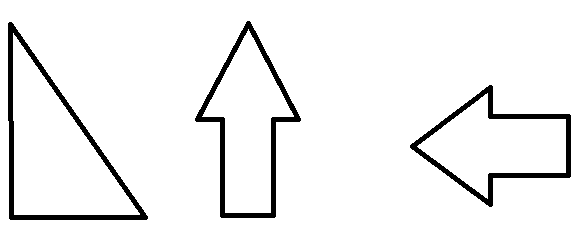
\includegraphics[scale=0.3]{mypicture.png}
\end{figure}


\subsection*{Kategorie}
\ifthenelse{\equal{\category}{give}}{$\boxtimes$}{$\Box$} Give \\
\ifthenelse{\equal{\category}{take}}{$\boxtimes$}{$\Box$} Take \\
\ifthenelse{\equal{\category}{exchange}}{$\boxtimes$}{$\Box$} Exchange \\
\ifthenelse{\equal{\category}{extend}}{$\boxtimes$}{$\Box$} Extend \\
\ifthenelse{\equal{\category}{connect}}{$\boxtimes$}{$\Box$} Connect



\section*{Wie}

\subsection*{Aktion des Benutzers}
\useraction

\subsection*{Reaktion des Sende-und Empfänger-Gerätes}
%\reaction

\subsection*{Hinweise zur Gestaltung der Interaktion}
%\designnotes



\section*{Wann}

\subsection*{Geeigneter Nutzungskontext}

\subsubsection*{Zeit}
\ifthenelse{\equal{\when}{gleichzeitig}}{$\boxtimes$}{$\Box$} gleichzeitige Nutzung von Geräten \\
\ifthenelse{\equal{\when}{aufeinanderfolgend}}{$\boxtimes$}{$\Box$} sequentielle Nutzung von Geräten 

\subsubsection*{Modus}
\ifthenelse{\equal{\mode}{online}}{$\boxtimes$}{$\Box$} online \\
\ifthenelse{\equal{\mode}{offline}}{$\boxtimes$}{$\Box$} offline \\

%\validcontext

\subsection*{Abzuratender Nutzungskontext}
%\notvalidcontext

\subsection*{Geräteklassen}
\begin{tabular}{|c|c|c|c|c|}
\hline 
• & • & Mittel & Riesig & Groß \\ 
\hline 
• & • & • & • & • \\ 
\hline 
• & • & • & • & • \\ 
\hline 
• & • & • & • & • \\ 
\hline 
• & • & • & • & • \\ 
\hline 
\end{tabular} 

\subsection*{Entfernung zwischen Sender- und Empfänger-Gerät}



\section*{Warum}


\subsection*{Displaygrößen}


\subsection*{Analoge Patterns}


\subsection*{State of the Art/Gebrauchshistorie}


\subsection*{Checkliste: Entspricht die Interaktion der Definiton eines "Blended Interaction"?}


\section*{Technisches}

\subsection*{Technologien zur Objekterkennung}


\subsection*{Technologien zur Kommunikation}


\subsection*{Technologien zur Bewegungs-/Orientierungsbestimmung}


\subsection*{Prototyp/Lösungsansatz/Code-Snippets/UML-Diagramm}



\section*{Sonstiges}

\subsection*{Autor/en}

\subsection*{Literaturreferenzen}

\subsection*{Abbildungsverzeichnis}

\subsection*{Versionshistorie}

\subsection*{Kommentare}

\subsection*{Offene Fragen}